\documentclass[11pt]{article}
\usepackage[margin=0.78in]{geometry}
\usepackage[T1]{fontenc}
\usepackage{lmodern}
\usepackage{microtype}
\usepackage{amsmath,amssymb,mathtools}
\usepackage{booktabs,longtable,tabularx,array}
\usepackage{enumitem}
\usepackage[dvipsnames,table]{xcolor}
\usepackage{graphicx}
\usepackage{tikz}
\usetikzlibrary{arrows.meta,positioning}
\usepackage{hyperref}
\hypersetup{colorlinks=true,linkcolor=NavyBlue,urlcolor=RoyalBlue}
\setlist{nosep,leftmargin=*}
\setlength{\parindent}{0pt}
\setlength{\parskip}{5pt}
\renewcommand{\arraystretch}{1.13}

\definecolor{exactgreen}{RGB}{221,243,226}
\definecolor{condblue}{RGB}{225,237,250}
\definecolor{compgold}{RGB}{255,243,207}
\definecolor{falsepink}{RGB}{253,225,229}
\definecolor{opengray}{RGB}{238,238,238}
\newcommand{\Exact}{\textsc{Proved/Exact}}
\newcommand{\Cond}{\textsc{Conditional}}
\newcommand{\Comp}{\textsc{Computational}}
\newcommand{\False}{\textsc{Falsified}}
\newcommand{\Open}{\textsc{Open}}

\title{FINAL-LINK2 Corpus Recovery Audit\\
\large Witness-Preserving Covers, Charged Acquisition, and the Missing Contractive Edge}
\author{Automated proof-recovery agent \texttt{FINAL-LINK-CORPUS}}
\date{Immutable run snapshot: 2026-10-08 01:01:35 UTC}

\begin{document}
\maketitle

\begin{abstract}
This report audits the local \texttt{pnp\_spines} corpus, the recovered WRAPPER archive, accessible Google Drive proof logs, and the GitHub snapshot \texttt{j15marti/pnp} for an overlooked theorem supplying the final COVER--SHRINK link.  The concrete target is an exact, source-checkable construction which, on every SAT encoding of size $M$, produces at most $M^{1/3+o(1)}$ recursively consumable children of size at most $M^{2/3+o(1)}$ in total charged work $M^{1+o(1)}$, with the required same-realization workspace.  Many exact components are recovered: portfolio composition, recurrence closure, lossless width-three reconstruction, clause-dominance selection, and an exponent ratchet that removes dependence on an initially unknown polynomial exponent.  None constructs the required cover.  Every apparent closure either assumes a contractive extractor such as CSE/LIOD/BatchAcquire/G2, holds only for a restricted fragment or supplied representation, counts one child rather than total fanout, or compresses the output only after paying the original SAT cost.
\end{abstract}

\section{Bottom-line determination}

\begin{center}
\fcolorbox{BrickRed}{falsepink}{\parbox{0.93\textwidth}{
\textbf{No recovered statement closes FINAL-LINK1.}  The remembered elimination of the $K$ exponent is real and exact, but it is a post-contraction recurrence theorem: once a uniformly iterable strict shrinker exists, repeated application drives the exponent to a fixed point independent of the starting $K$.  It does not construct the first shrinker or pay for acquiring its source-dependent summaries.
}}
\end{center}

The strongest defensible present claim is this conditional normal form.

\textbf{Conditional FINAL-LINK normal form.}
Fix a deterministic exact SAT decider $A$.  Suppose a fixed finite family of $A$-dependent partial procedures has these properties on every sufficiently large source $F$ of encoded size $M$:
\begin{enumerate}
  \item each procedure either returns a verifiably safe \textsc{fail} or an exact witness-preserving recursive plan;
  \item at least one procedure succeeds on every $F$;
  \item after charging all attempts, source reads, summary construction, normalization, replay, and aggregation, the combined plan has
  \[
       q(F)\le M^{1/3+o(1)},\qquad
       \max_i |F_i|\le M^{2/3+o(1)},\qquad
       W(F)\le M^{1+o(1)};
  \]
  \item the children are ordinary instances in the same recursive model, no current-scale call to $A$ is hidden in construction or access, and time and workspace hold on the same realization.
\end{enumerate}
Then \textsc{CERTIFIED-PARTIAL-PORTFOLIO1} combines the routes, and \textsc{RECURCLOSE1}/\textsc{PRF2-0155} removes the original exponent $K$.  This implication is exact.  Items 2--4 are the missing theorem, not an already proved lemma.

\section{Target and accounting}

For a source formula $F$ of length $M$, write a proposed exact reduction as
\[
  F \longmapsto \bigl(D;\,F_1,\ldots,F_q\bigr),
\]
where $D$ is charged metadata and the answers to the $F_i$ combine to the exact answer for $F$, with witness lifting wherever claimed.  The target is
\begin{equation}
\label{eq:target}
  q\le M^{1/3+o(1)},\qquad |F_i|\le M^{2/3+o(1)},\qquad
  W_{\rm all}\le M^{1+o(1)}.
\end{equation}
The product $q\max_i|F_i|\le M^{1+o(1)}$ lies exactly on the explicit-output-volume boundary.  Linear-time production is therefore not ruled out by output length.  The missing part is a general exact semantic decomposition whose interfaces do not reintroduce the source computation.

For a recursively closed transformation with $q=M^{\eta+o(1)}$, child scale $M^{\theta+o(1)}$, $\theta<1$, and local work $M^{r+o(1)}$, the recovered recurrence is
\begin{equation}
\label{eq:recurrence}
  T(M)\le M^{r+o(1)}+M^{\eta+o(1)}T(M^{\theta+o(1)}),
  \qquad
  \operatorname{exp}(T)\le \max\left\{r,\frac{\eta}{1-\theta}\right\}.
\end{equation}
At $(\eta,\theta,r)=(1/3,2/3,1)$ the fixed point is $1$.  This is the valid location of the original division intuition: repeated multiplicative contraction removes the starting exponent only after a charged, recursively iterable contraction is supplied.

\section{Dependency graph}

\begin{figure}[ht]
\centering
\resizebox{\textwidth}{!}{%
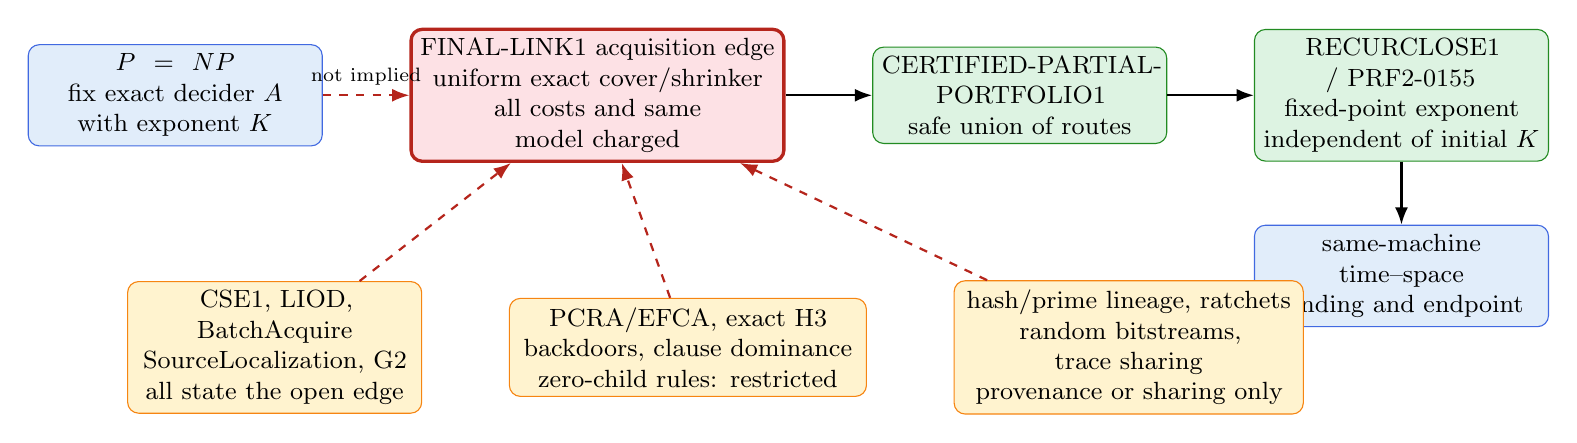
\begin{tikzpicture}[
  node distance=8mm and 11mm,
  box/.style={draw,rounded corners,align=center,minimum height=10mm,text width=35mm,font=\small},
  exact/.style={box,fill=exactgreen,draw=ForestGreen},
  cond/.style={box,fill=condblue,draw=RoyalBlue},
  open/.style={box,fill=falsepink,draw=BrickRed,very thick},
  restricted/.style={box,fill=compgold,draw=BurntOrange},
  arr/.style={-{Latex[length=2.2mm]},thick},
  gap/.style={-{Latex[length=2.2mm]},thick,dashed,draw=BrickRed}
]
\node[cond] (pnp) {$P=NP$\\fix exact decider $A$\\with exponent $K$};
\node[open,right=of pnp,text width=45mm] (extract) {FINAL-LINK1 acquisition edge\\uniform exact cover/shrinker\\all costs and same model charged};
\node[exact,right=of extract] (portfolio) {CERTIFIED-PARTIAL-\\PORTFOLIO1\\safe union of routes};
\node[exact,right=of portfolio] (recur) {RECURCLOSE1 / PRF2-0155\\fixed-point exponent\\independent of initial $K$};
\node[cond,below=of recur] (landing) {same-machine time--space\\landing and endpoint};
\node[restricted,below=15mm of extract,xshift=-41mm] (c1) {CSE1, LIOD, BatchAcquire\\SourceLocalization, G2\\all state the open edge};
\node[restricted,right=of c1,text width=43mm] (c2) {PCRA/EFCA, exact H3\\backdoors, clause dominance\\zero-child rules: restricted};
\node[restricted,right=of c2,text width=42mm] (c3) {hash/prime lineage, ratchets\\random bitstreams, trace sharing\\provenance or sharing only};
\draw[gap] (pnp) -- node[above,font=\scriptsize]{not implied} (extract);
\draw[arr] (extract) -- (portfolio);
\draw[arr] (portfolio) -- (recur);
\draw[arr] (recur) -- (landing);
\draw[gap] (c1) -- (extract);
\draw[gap] (c2) -- (extract);
\draw[gap] (c3) -- (extract);
\end{tikzpicture}}
\caption{All downstream arrows are exact once the red acquisition node is assumed.  The lower boxes supply controls, counterexamples, or reformulations; none proves the dashed edge.}
\end{figure}

\section{Evidence matrix}

\small
\begin{longtable}{p{0.17\textwidth}p{0.14\textwidth}p{0.39\textwidth}p{0.18\textwidth}}
\toprule
\textbf{Item} & \textbf{Status} & \textbf{Established statement} & \textbf{Effect on FINAL-LINK1}\\
\midrule
\endfirsthead
\toprule
\textbf{Item} & \textbf{Status} & \textbf{Established statement} & \textbf{Effect on FINAL-LINK1}\\
\midrule
\endhead
\rowcolor{exactgreen}
RECURCLOSE1 & \Exact & A uniform recursive map with local exponent $r$, fanout exponent $\eta$, and child exponent $\theta<1$ has time exponent at most $\max\{r,\eta/(1-\theta)\}$. & Closes recursion only after the shrinker is supplied.\\
\rowcolor{exactgreen}
PRF2-0155 ratchet & \Exact & An iterable map $a\mapsto\lambda a+K_0$, $0<\lambda<1$, approaches $K_0/(1-\lambda)$ independently of starting $a$. & This is the recovered removal of $K$; transformer existence is a hypothesis.\\
\rowcolor{exactgreen}
CERTIFIED-PARTIAL-PORTFOLIO1 & \Exact & Fixed safe-fail/exact partial procedures combine if all inputs are covered and all attempts are charged. & Removes route selection but assumes coverage and resource bounds.\\
\rowcolor{exactgreen}
CLAUSE-DOM-SELECT1 & \Exact & If same-variable clause sets satisfy $R_2\subseteq R_1$, then $\operatorname{SAT}(R_1)\lor\operatorname{SAT}(R_2)=\operatorname{SAT}(R_2)$. & Query-free selector; no general density theorem.\\
\rowcolor{exactgreen}
CLAUSE-DOM-ANTICHAIN1 & \Exact & Complete unit-assignment formulas form an exponential pairwise-incomparable family. & Dominance alone cannot guarantee progress.\\
\rowcolor{exactgreen}
ZERO-CHILD-PORTFOLIO1 & \Exact & Cheap recognized domains may return an exact zero-child plan. & Restricted direct decision is not a general cover.\\
\rowcolor{exactgreen}
Width-three reconstruction & \Exact & A 3-CNF solution relation equals the intersection of all projections on at most three coordinates; supplied exact H3 compiles to polynomial 3-CNF. & General H3 acquisition is circular/current-scale; output need not shrink.\\
\rowcolor{exactgreen}
Wrapper path exposure & \Exact & WRAPPED-SELFRED1 exposes and replays an exact decision path; lineage is compact after contraction. & Raw aggregate cost is current-scale or worse; no $\theta<1$ query.\\
\rowcolor{exactgreen}
General semantic compression & \Exact & Under $P=NP$, run $A(F)$ and emit a constant YES/NO CNF. & Tiny output, but construction already costs $M^{K+o(1)}$.\\
\rowcolor{exactgreen}
VIRTUAL-CHILD-SPACE1 & \Cond & A child already known to be $M^\theta$ with a cheap bit transducer can be evaluated virtually within child-space plus metadata. & Does not construct or locally address that child.\\

\rowcolor{condblue}
CSE1 & \Cond & Contractive Source Extraction is specified with fractional objects, full acquisition charge, covariance, and recursive closure. & This specification is essentially FINAL-LINK1; construction is open.\\
\rowcolor{condblue}
LIOD & \Cond & A witness-relative on-demand interface would handle child-call space and source matching. & No charged low-space acquisition theorem.\\
\rowcolor{condblue}
BatchAcquire/global $H$ & \Cond & Cheap shared acquisition, boundary recovery, total batching, covariance, and compose/project would amortize the cover. & All conditions are explicit; existence is unproved.\\
\rowcolor{condblue}
SourceLocalization & \Cond & One-child arithmetic $\beta+\lambda K$ can beat a frontier; sparse all-child covers would work if irrelevant source data were certified. & Global fanout correction defeats the favored half-scale cell.\\
\rowcolor{condblue}
PCRA/EFCA & \Cond & Projection/composition/forget/label reset compactly for affine and bijunctive controls. & General-CNF effective reset and peak-size bound are open.\\
\rowcolor{condblue}
ORACLE-INCOMPLETE-BUT-RECURSIVELY-COMPLETE & \Cond & Incomplete smaller-query answers can compose to completeness if strict shrink and recursive closure hold. & Architecture only; it assumes the shrinker.\\
\rowcolor{condblue}
ARC/max-affine successor & \Cond & Contractive affine exponent maps have exact fixed points; typed cycles work if every return-cycle product is below one. & Broadens the sufficient region, but no all-input successor was recovered.\\

\rowcolor{compgold}
FINAL-LINK-HYBRID1 & \Comp & Finite heterogeneous tests verified semantics and many shape predicates. & Worst observed work was strongly superlinear; no asymptotic coverage.\\
\rowcolor{compgold}
Width-two census & \Comp & Reported 12,616 width-two formulas were settled by partial zero-child rules. & Finite/restricted validation.\\
\rowcolor{compgold}
Hash/bitstream/\allowbreak ratchet tests & \Comp & Fixed hash lengths, commitments, and prime lineage detect replay/collision/provenance faults. & Bind histories; do not contract SAT semantics.\\

\rowcolor{falsepink}
Half-scale all-block SourceLocalization & \False & Total exponent is $1-\lambda+\beta+\lambda K=1+\beta+\lambda(K-1)$. & At $K=2,\lambda=1/2$, cannot be below $4/3$, even as $\beta\to0$.\\
\rowcolor{falsepink}
Small term count implies small residual & \False & BDNF-WRAPPER-GATE1 has subpolynomially many terms and a residual of size $M^{1-o(1)}$. & Backdoor/disjunctive term count is not a child-size bound.\\
\rowcolor{falsepink}
Trace as global summary & \False & A realized trace answers only its realized trajectory. & It omits counterfactual restrictions needed by children.\\
\rowcolor{falsepink}
H3 nonemptiness as hard consumer & \False & Under the promised nonempty exact network, NONEMPTY-H3 is trivially YES. & Model finding/deep extension remains SAT on the compiled network.\\
\rowcolor{falsepink}
Memoization alone contracts & \False & Sharing exact repeats removes duplicates, not unique probes, states, or regenerated children. & No universal repetition/density theorem.\\

\rowcolor{opengray}
All-input cover/shrinker & \Open & Exact general construction satisfying Equation~\ref{eq:target}, source matching, and recursive closure. & This is FINAL-LINK1.\\
\rowcolor{opengray}
General cheap acquisition & \Open & Obtain summaries/labels/interfaces before a parent-scale SAT computation. & Shared premise of CSE, LIOD, BatchAcquire, G2, and general EFCA.\\
\rowcolor{opengray}
Same-realization landing & \Open & Time and workspace, including metadata/regeneration, must hold for one machine/run. & Separate time and space witnesses do not compose.\\
\bottomrule
\end{longtable}
\normalsize

\section{Recovered components and exact limitations}

\subsection{CSE and LIOD name the missing interface}

GitHub \texttt{main2.tex}/\texttt{main3.tex} define Contractive Source Extraction (CSE) by asking, for every deterministic exact decider $A$ and sufficiently large hard scale $N$, for recursively consumable source-matched objects with fractional count, live support exponent below one, fully charged acquisition/combination, wrapper covariance, recursive closure, and no hidden current-scale SAT call.  The associated audits explicitly mark CSE1 open.  WRAPPED-SELFRED1 gives an exact exposed path, but its recovered ledger is $\Theta(n^{K+1})$, contains no $\theta<1$ recursive query, and does not eliminate $K$.

LIOD is a witness-relative form of the same edge.  The archive says the interface handles child-call space only after a LIOD-like coverage theorem exists.  It also records an important quantifier guard: an extensional schema using only smaller SAT answers and uniformly recursively applicable yields an unconditional polynomial SAT algorithm.  A hypothesis-dependent construction therefore needs $A$-specific intensional data, whose acquisition must be charged.  No recovered LIOD candidate supplies it.

\subsection{BatchAcquire and shared global $H$}

The most precise positive contract requires $H=H(A,F,B)$ to satisfy:
\begin{enumerate}
  \item acquisition in $M^{h+o(1)}$ time and controlled space below the parent-scale cost;
  \item recovery of every boundary label from $(H,z)$ in $M^{r+o(1)}$;
  \item total generation of all $M^\beta$ labels/accessors in the claimed shared bound;
  \item covariance under the wrapper after charged normalization;
  \item recursive COMPOSE/PROJECT without rereading the parent source.
\end{enumerate}
The source explicitly says this is unproved and gives a counterexample taxonomy.  Source-as-$H$ has cheap acquisition but parent-scale recovery.  Answer-table-as-$H$ has cheap recovery but unexplained acquisition.  Trace-as-$H$ lacks counterfactual branches.  MUX/pointer access makes lookup cheap, not adaptive composition.  Circuit-as-$H$ is cheap to acquire but leaves circuit evaluation; adding gate values moves the cost into acquisition.  BatchAcquire is therefore a clean specification, not a constructor.

\subsection{SourceLocalization correction}

For one child of scale $M^\lambda$ and acquisition factor $M^\beta$, inherited exponent $K$ gives $\beta+\lambda K$.  Thus the archived $(K,C,\lambda,\beta)=(2,4/3,1/2,<1/6)$ cell is favorable for one child.

For an all-block cover with $M^{1-\lambda}$ children, total exponent is
\[
 (1-\lambda)+\beta+\lambda K=1+\beta+\lambda(K-1).
\]
At $K=2,\lambda=1/2$ this is $3/2+\beta$, not below $4/3$.  With fanout exponent $a$, the cost is $a+\beta+\lambda K$.  An explicit cover of all $\Theta(M)$ source items also has $a+\lambda\ge1$.  A sparse cover needs an implicit/shared representation, answer-dependent safe selection, or a theorem that most source data are irrelevant.  Each escape is separately marked open and must include acquisition/replay.

\subsection{H3, G2, and PCRA/EFCA}

For a 3-CNF relation $R=\operatorname{Sol}(F)$, the archive proves
\[
 R=\bigcap_{|J|\le3}\operatorname{Cyl}(\pi_J(R)).
\]
Given exact H3, forbidden local tuples compile to polynomial-size 3-CNF.  But $F\mapsto H3(F)$ asks whether each local tuple extends to a global satisfying assignment: SAT extension queries.  This is G2, explicitly open.  A full H3 also has $\Theta(n^3)$ local tables, linear in a dense $M\asymp n^3$ encoding and expansive for sparse $M\asymp n$.  It need not meet the $M^{2/3}$ child target even when supplied.

PCRA and the weakened EFCA formulation correctly charge REPRESENT, COMPOSE, FORGET, LABEL, intermediate peak size, time, and space.  Affine and bijunctive relations are positive controls.  No general-CNF theorem is present.  Repeated normalization $s_{j+1}\le s_j^d$, $d>1$, can blow up over $\Theta(\log M)$ levels.  H3/PCRA is a restricted route whose general acquisition/reset hypothesis remains open.

\subsection{Selectors, zero-child rules, backdoors, and disjunctions}

Clause dominance is a genuinely free selector once inclusion is known; the exact antichain construction prevents a universal progress claim.  RUP/nested implication variants likewise lack a general density theorem.

ZERO-CHILD-PORTFOLIO1 is exact on cheaply recognized, directly decided domains.  CERTIFIED-PARTIAL-PORTFOLIO1 safely unions those routes.  It still requires every input to have a successful route and charges every attempt.  A backdoor $B$ gives the exact cover
\[
  \operatorname{SAT}(F)=\bigvee_{\alpha\in\{0,1\}^{B}}
  \operatorname{SAT}(F\!\upharpoonright\!\alpha),
\]
but only helps if $B$ is cheaply found, sufficiently small, and all residuals contract.  BDNF-WRAPPER-GATE1 refutes the inference from few terms to small residual.  Clause-first branching has constant fanout per level but can require linear depth and exponential leaves.  Parallel wrappers add routes, not universal coverage.

\subsection{Hashes, random bitstreams, lineage, and sharing}

Four-, six-, or eight-hex-digit hashes alter finite collision and storage rates.  Exact replay still needs collision-free identity or charged verification.  Response signatures, ratchets, and bitstreams bind causal order under a no-new-source-information cut.  Prime lineage gives an ordered $O(T\log T)$ code, and macro-lineage may be logarithmic after a contraction bounds $T$.  None changes the SAT relation or proves a smaller child.

The corpus uses CSE in two senses.  Contractive Source Extraction is the open interface.  Ordinary common-subexpression elimination memoizes repeated DAG nodes.  The latter can improve an upper bound but no theorem guarantees enough repetition on every wrapper trace.  Unique probes, local operations, state, and regeneration remain charged.

\section{Logically valid syntheses attempted}

\subsection{A. Partial portfolio plus recurrence}

Let a fixed finite family safely fail or return exact plans.  If combined attempt cost is $M^{1+o(1)}$, every source is accepted, and every accepted plan meets Equation~\ref{eq:target} with recursive closure, portfolio composition and Equation~\ref{eq:recurrence} give time $M^{1+o(1)}$.  This synthesis is exact.  The corpus supplies several members---dominance, easy zero-child domains, backdoors, and restricted PCRA/H3 controls---but no coverage proof.  Replacing all-input coverage by all tested instances is the finite-to-asymptotic quantifier error.

\subsection{B. Shared $H$ at the output-volume boundary}

Suppose $H$ is acquired in $M^{1+o(1)}$ total work and generates $M^{1/3+o(1)}$ exact child descriptions of length $M^{2/3+o(1)}$, with aggregate recovery/replay also linear, recursive closure, and no parent rereads.  The product is $M^{1+o(1)}$, so explicit emission fits the budget and recurrence closes.  This is the cleanest composition, but its premise is exactly BatchAcquire/CSE.  The source-, answer-table-, and trace-as-$H$ examples show that cheap acquisition or cheap lookup alone is insufficient.

\subsection{C. H3 reconstruction plus shared acquisition}

One can use a supplied exact H3 as $H$, compile local constraints, and compose via PCRA/EFCA.  The semantics are exact under the promise.  The map $F\mapsto H3(F)$ is G2, the missing current-scale computation, and the representation need not shrink.  This synthesis assumes the gap twice.

\subsection{D. SourceLocalization plus sparse selection}

The one-child calculation could sit in a portfolio selecting only $M^{1/3}$ half-scale candidates while a shared summary supplies omitted consistency.  This is numerically promising.  Certifying unselected blocks as irrelevant is the absent SourceLocalization theorem; supplying their effects is BatchAcquire.  The composition is valid if assumed, not an independent derivation.

\subsection{E. Restricted algebra union}

The union of affine EFCA, bijunctive EFCA, recognized zero-child rules, favorable backdoors, and dominance selectors is an exact solver for the union of recognized domains, with maximum charged cost.  No theorem says this union contains every CNF.  It is a useful achievable-region result and test framework, not general SAT compression.

\subsection{F. Decide then emit}

Under $P=NP$, decide $F$ with $A$ and emit a constant YES/NO formula.  It achieves $q=1$ and constant child size but pays $M^{K+o(1)}$ first.  Recursing on the tiny output cannot erase the parent cost.  This is the canonical output-compression versus acquisition mismatch.

\subsection{G. Alternative ARC/max-affine route}

The numerical cell is sufficient, not necessary.  For
\[
  t'\le\max\left(r,\max_j(w_j+\lambda_jt)\right),\qquad
  s'\le\max\left(p,\max_j\lambda_js\right),
\]
with every recursive return-cycle product below one, the exact fixed point is controlled by $\max(r,\max_j w_j/(1-\lambda_j))$ and $p$.  A route below the endpoint could close the spine without Equation~\ref{eq:target} literally.  The corpus still has no all-input strict successor with fully charged $w_j,r,p$ and same-model closure.  ARC broadens the search region; it does not supply an overlooked proof.

\section{Quantifier and model mismatch audit}

\begin{longtable}{p{0.28\textwidth}p{0.30\textwidth}p{0.345\textwidth}}
\toprule
\textbf{Tempting inference} & \textbf{Mismatch} & \textbf{Required repair}\\
\midrule
\endfirsthead
\toprule
\textbf{Tempting inference} & \textbf{Mismatch} & \textbf{Required repair}\\
\midrule
\endhead
A compact summary exists. & $\exists H$ versus a uniform algorithm constructing $H$ before solving the source. & State ACQUIRE, time/space, and every source access.\\
Each child is cheap. & Per-child cost versus the sum over $q$ children. & Charge $q$ recoveries or prove a shared batch bound.\\
One child beats the frontier. & One route versus an exact cover of all satisfying possibilities. & Charge fanout; prove safe selection or combination.\\
It works for affine, 2-SAT, or supplied H3. & Restricted fragment/promise versus every CNF. & Give a charged general extractor or retain the restriction.\\
Every input has some route. & Nonuniform existence versus one fixed finite machine. & Safe failure, fixed portfolio, bounded attempts, full coverage.\\
$P=NP$ supplies an algorithm. & Some exponent $K$ versus a successor contractive in $K$. & Prove the successor, then apply the ratchet.\\
The output is small. & Representation length versus acquisition, recovery, normalization, aggregation. & Charge the entire compiler and replay.\\
The trace has the answers. & One realized path versus counterfactual child restrictions. & Provide a covariant boundary interface.\\
SAT values are preserved. & Answer equality versus witness lifting, source matching, valid syntax. & Specify combiner, lifting, and child encoding.\\
The child is virtual. & Read-only oracle access versus ordinary single-input RAM. & Charge bit generation and justify the endpoint model.\\
Best time and best space are known. & Possibly different algorithms/runs versus one realization. & Attach both ledgers to the same machine.\\
All experiments pass. & Finite census versus asymptotic universal statement. & Prove a source-checkable invariant for all lengths.\\
H3 is nonempty. & Promise-YES nonemptiness versus general SAT/model finding. & Handle NO networks and deep extension without hidden SAT.\\
Only smaller SAT answers are used. & Extensional black-box schema versus $A$-specific intensional data. & Explain and charge how $A$ enters, or accept unconditional recursion.\\
Children share the source. & Handle length versus aggregate shared-source traffic. & Charge reads, cache state, regeneration, covariance.\\
\bottomrule
\end{longtable}

\section{Computational evidence}

The computational artifacts are valuable falsification tools: they verify bounded semantics, expose selector mistakes, and locate resource blowups.  They do not replace an all-input invariant.

A later FINAL-LINK-HYBRID1 builder run reported shape success on 27 heterogeneous cases and no semantic errors, but observed work up to 3,518,492 operations for $M=2,282$, an empirical exponent near $1.95$; work was not part of the recorded shape-success predicate.  An earlier proof report tested 34 heterogeneous cases, with one incomplete shape case; none met the desired $M^{2/3}$ explicit-workspace scale, though some met a looser $M^{4/3}$ diagnostic.  These results support the portfolio architecture while warning that acquisition and workspace remain unproved.

Hash/ratchet and XOR-wrapper experiments likewise found and repaired finite semantic failures.  Nearby satisfiable perturbations of structured families remained uncovered in red-team testing.  The proper classification is \Comp{} support for testing and counterexample discovery, not a proof of general compression.

\section{Precise remaining theorem}

\begin{center}
\fcolorbox{BrickRed}{opengray}{\parbox{0.92\textwidth}{
\textbf{FINAL-LINK1 (charged witness-preserving cover).}  For the selected exact decider $A$ (or the precisely declared source-only model), construct on every sufficiently large CNF $F$ of length $M$ an exact recursive plan with at most $M^{1/3+o(1)}$ ordinary children, each of length at most $M^{2/3+o(1)}$.  The complete construction---discovery, failed routes, source reads, summaries, labels, normalization, witness lifting, aggregation, and replay---uses $M^{1+o(1)}$ time and the claimed same-realization workspace.  It is wrapper-covariant, closes recursively without parent rereading, and makes no hidden current-scale call to $A$.
}}
\end{center}

An ARC theorem may replace the numeric cell if its max-affine fixed point plus workspace lies below the endpoint, but it must satisfy the same acquisition, quantifier, and model requirements.  Either statement is a substantial new theorem: a solver-independent FINAL-LINK1 already implies near-linear SAT by Equation~\ref{eq:recurrence}.

\section{Conclusions}

\begin{enumerate}
  \item The downstream spine is coherent: exact partial routes combine; strict contraction removes the unknown $K$; an appropriate same-machine time--space landing can then be applied.
  \item The original division intuition belongs at recurrence closure, not cover construction.  It explains why contraction is powerful but cannot prove contraction exists.
  \item CSE, LIOD, BatchAcquire, SourceLocalization, G2, general EFCA, and ORACLE-INCOMPLETE-BUT-RECURSIVELY-COMPLETE are illuminating formulations of the unresolved edge.  None is an established constructor.
  \item Dominance, zero-child rules, restricted algebras, backdoors, disjunctive wrappers, hashes, ratchets, random bitstreams, and DAG sharing are valid components or tests.  Their hypotheses do not cover arbitrary CNF with the target ledger.
  \item No recovered composition proves Equation~\ref{eq:target}.  The strongest defensible manuscript should keep the result conditional and mark acquisition plus coverage OPEN.
\end{enumerate}

\section*{Source inventory}
\vspace{-15pt}

\begingroup
\scriptsize
\begin{itemize}
  \item Local corpus root: \path{/workspace/scratch/6224f8f6ab8c/pnp_spines}.
  \item Prior audit: \path{research/agents/research/2026-10-08_003226_FINAL-LINK-CORPUS.tex}.
  \item Hash recovery: \path{research/agents/research/2026-10-07_2345_CORPUS_HASH_RECOVERY.tex}.
  \item Hybrid report: \path{research/agents/proof/2026-10-08_003700_PROOF_FINAL-LINK-HYBRID1.tex}.
  \item ARC audit: \path{research/agents/lead/2026-10-08_0032_LEAD_FINAL-LINK-ARC.tex}.
  \item Wrapper comparison: \path{wrapper_bound_match.tex}.
  \item GitHub: \url{https://github.com/j15marti/pnp}; especially \texttt{main2.tex}, \texttt{main3.tex}, and the recovered CSE, locality, virtual-child, and Williams-endpoint audits dated 2026-10-06.
  \item Drive SourceLocalization log (document ID):\\
    \texttt{17Lq\_mvPtU8GvdCP\_szj9lXheM1yLUIgCCV8Q1wM-YUU}.
  \item Drive exponent-ratchet log (document ID):\\
    \texttt{1gp-Q7IPCAioAv2iByQC5a12NDw98-v-F13ivxkKX0iI}.
  \item Library: \texttt{WRAPPER\_PROVED\_audit\_2026-10-07.json} (LIOD/PCRA/H3/BatchAcquire excerpts).
\end{itemize}
\endgroup

\end{document}
